\section{Image\-Detial Class Reference}
\label{classImageDetial}\index{ImageDetial@{ImageDetial}}
{\tt \#include $<$imagedetial.h$>$}

Inheritance diagram for Image\-Detial:\begin{figure}[H]
\begin{center}
\leavevmode
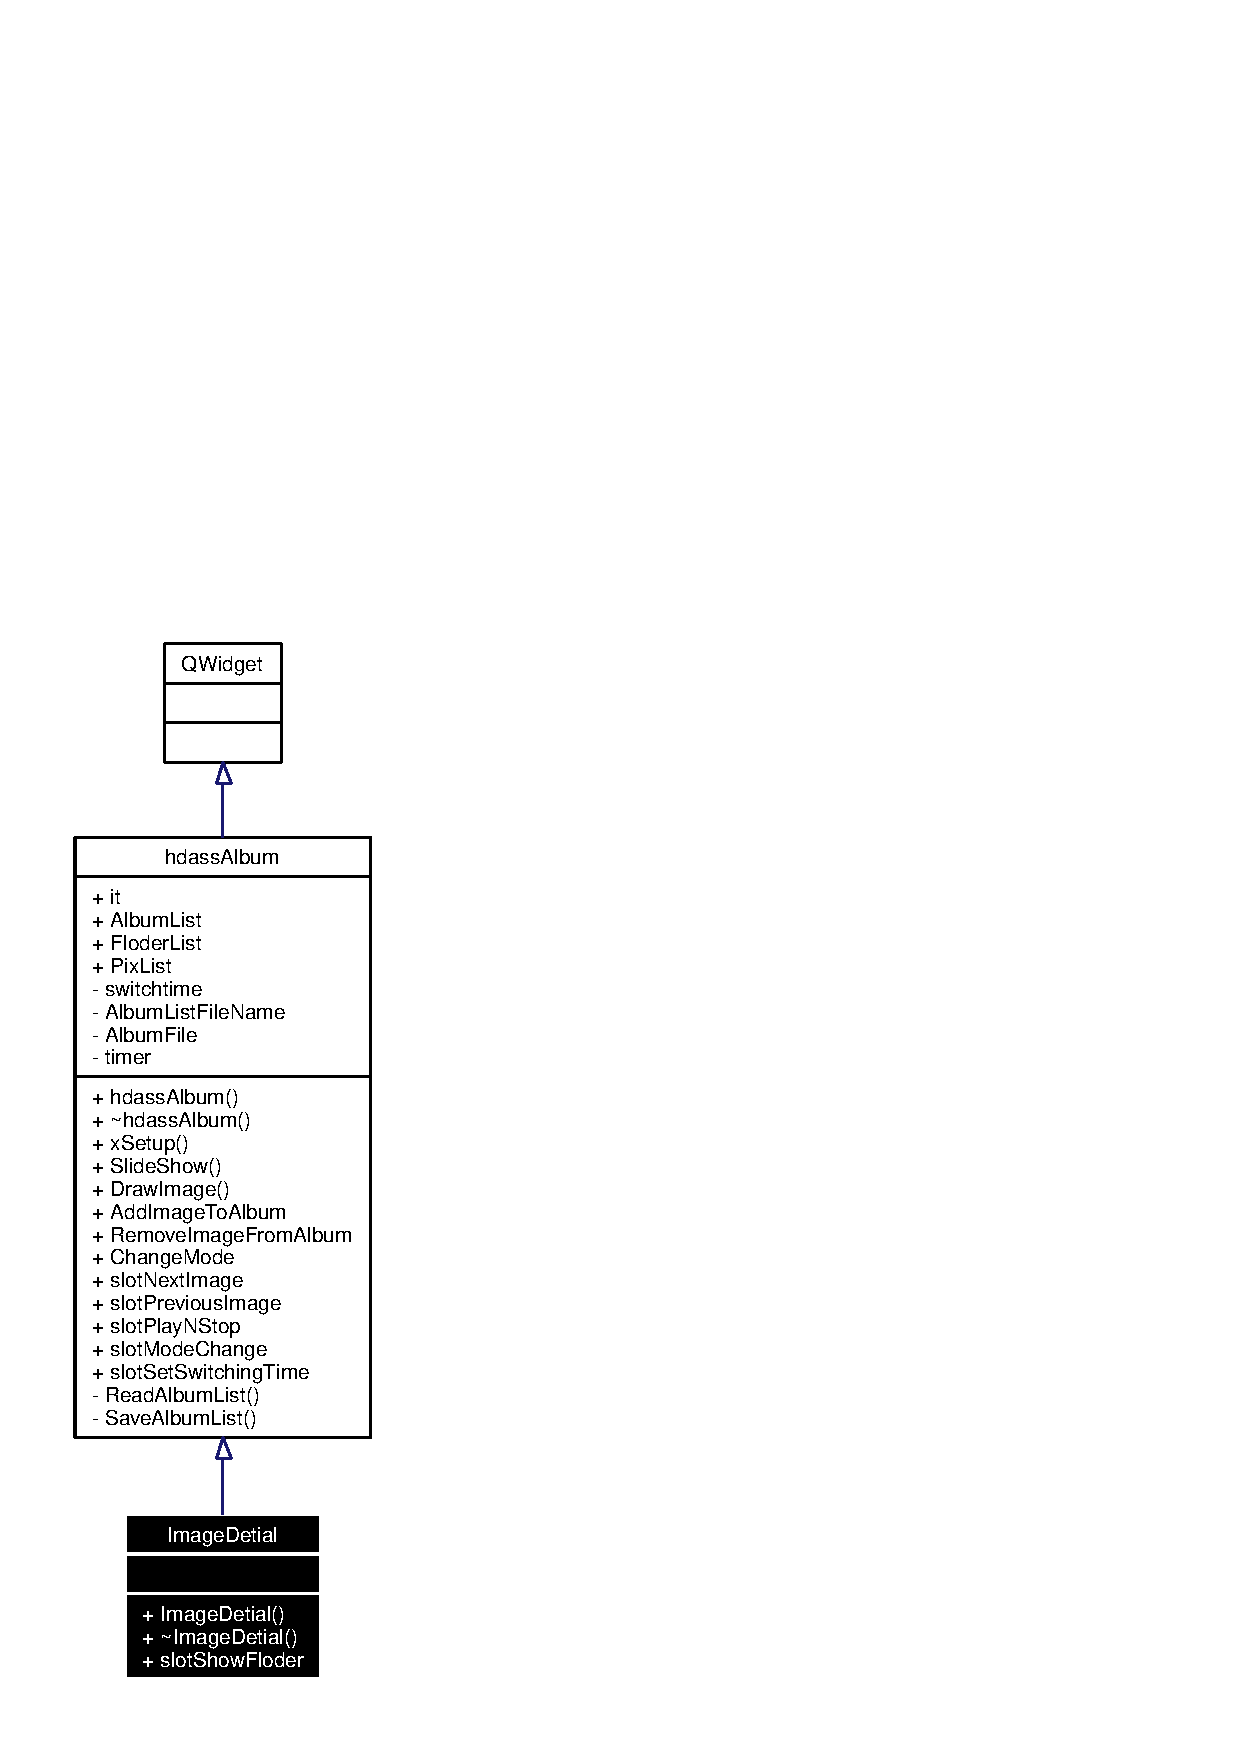
\includegraphics[width=89pt]{classImageDetial__inherit__graph}
\end{center}
\end{figure}
Collaboration diagram for Image\-Detial:\begin{figure}[H]
\begin{center}
\leavevmode
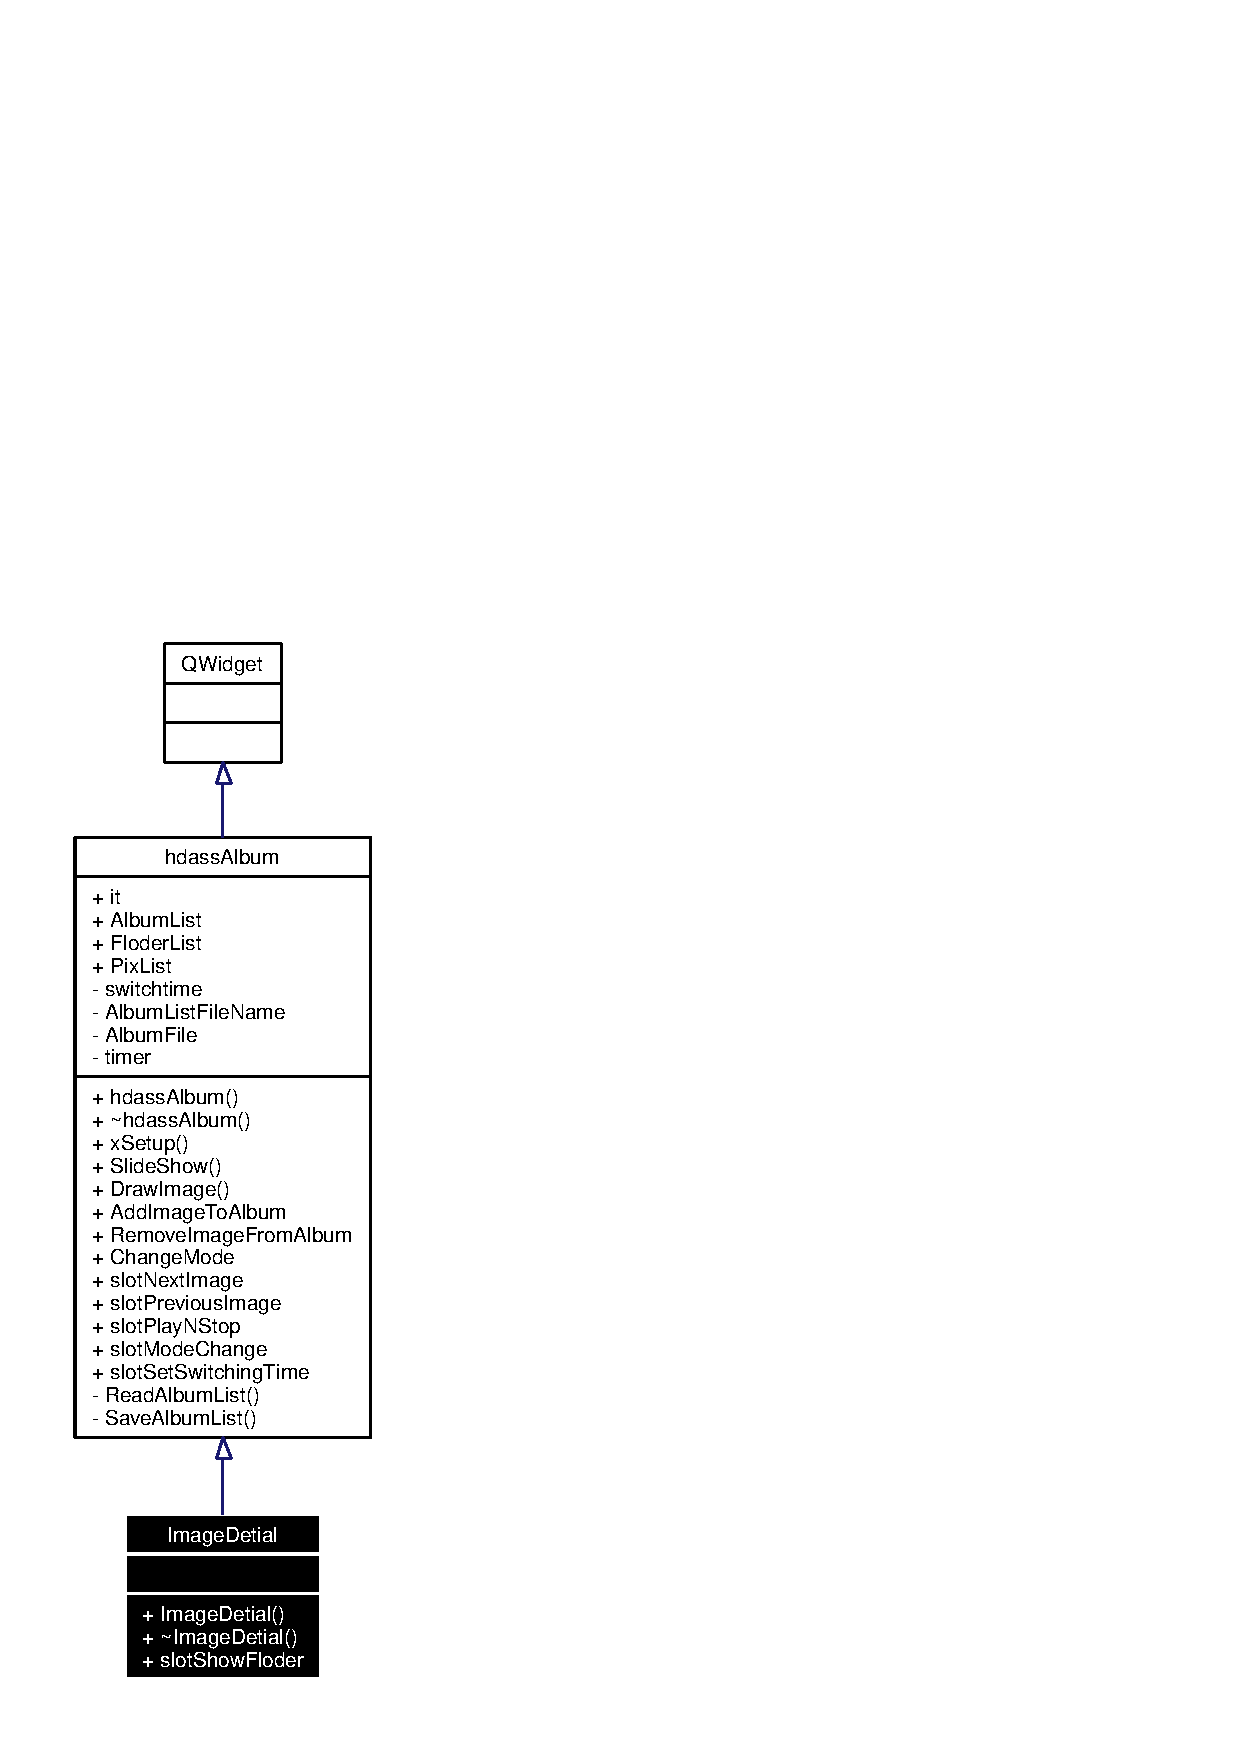
\includegraphics[width=89pt]{classImageDetial__coll__graph}
\end{center}
\end{figure}


\subsection{Detailed Description}
\begin{Desc}
\item[Author:]sonicat \end{Desc}




Definition at line 28 of file imagedetial.h.\subsection*{Public Slots}
\begin{CompactItemize}
\item 
void {\bf slot\-Show\-Floder} (KURL floder\_\-file)
\item 
void {\bf Add\-Image\-To\-Album} (KURL addimage)
\item 
void {\bf Remove\-Image\-From\-Album} (KURL removeimage)
\item 
void {\bf Change\-Mode} ({\bf Album\-Mode} mode)
\item 
void {\bf slot\-Next\-Image} ()
\item 
void {\bf slot\-Previous\-Image} ()
\item 
void {\bf slot\-Play\-NStop} ()
\item 
void {\bf slot\-Mode\-Change} (int)
\item 
void {\bf slot\-Set\-Switching\-Time} (int time)
\end{CompactItemize}
\subsection*{Public Member Functions}
\begin{CompactItemize}
\item 
{\bf Image\-Detial} ({\bf QWidget} $\ast$parent=0, const char $\ast$name=0)
\item 
{\bf $\sim$Image\-Detial} ()
\item 
void {\bf x\-Setup} ()
\item 
void {\bf Slide\-Show} ()
\item 
void {\bf Draw\-Image} (QPixmap pix)
\end{CompactItemize}
\subsection*{Public Attributes}
\begin{CompactItemize}
\item 
KURL::List::Const\-Iterator {\bf it}
\item 
KURL::List {\bf Album\-List}
\item 
KURL::List {\bf Floder\-List}
\item 
QPtr\-List$<$ QPixmap $>$ {\bf Pix\-List}
\end{CompactItemize}


\subsection{Constructor \& Destructor Documentation}
\index{ImageDetial@{Image\-Detial}!ImageDetial@{ImageDetial}}
\index{ImageDetial@{ImageDetial}!ImageDetial@{Image\-Detial}}
\subsubsection{\setlength{\rightskip}{0pt plus 5cm}Image\-Detial::Image\-Detial ({\bf QWidget} $\ast$ {\em parent} = 0, const char $\ast$ {\em name} = 0)}\label{classImageDetial_ImageDetiala0}




Definition at line 22 of file imagedetial.cpp.



\footnotesize\begin{verbatim}23  : hdassAlbum(parent, name)
24 {
25 }
\end{verbatim}\normalsize 
\index{ImageDetial@{Image\-Detial}!~ImageDetial@{$\sim$ImageDetial}}
\index{~ImageDetial@{$\sim$ImageDetial}!ImageDetial@{Image\-Detial}}
\subsubsection{\setlength{\rightskip}{0pt plus 5cm}Image\-Detial::$\sim${\bf Image\-Detial} ()}\label{classImageDetial_ImageDetiala1}




Definition at line 28 of file imagedetial.cpp.



\footnotesize\begin{verbatim}29 {
30 }
\end{verbatim}\normalsize 


\subsection{Member Function Documentation}
\index{ImageDetial@{Image\-Detial}!AddImageToAlbum@{AddImageToAlbum}}
\index{AddImageToAlbum@{AddImageToAlbum}!ImageDetial@{Image\-Detial}}
\subsubsection{\setlength{\rightskip}{0pt plus 5cm}void hdass\-Album::Add\-Image\-To\-Album (KURL {\em addimage})\hspace{0.3cm}{\tt  [slot, inherited]}}\label{classhdassAlbum_ImageDetiali1}




Definition at line 60 of file hdassalbum.cpp.

References hdass\-Album::Album\-List.



\footnotesize\begin{verbatim}61 {
62    AlbumList<<addimage;
63 }
\end{verbatim}\normalsize 
\index{ImageDetial@{Image\-Detial}!ChangeMode@{ChangeMode}}
\index{ChangeMode@{ChangeMode}!ImageDetial@{Image\-Detial}}
\subsubsection{\setlength{\rightskip}{0pt plus 5cm}void hdass\-Album::Change\-Mode ({\bf Album\-Mode} {\em mode})\hspace{0.3cm}{\tt  [slot, inherited]}}\label{classhdassAlbum_ImageDetiali3}




Definition at line 69 of file hdassalbum.cpp.



\footnotesize\begin{verbatim}70 {
71 
72 }
\end{verbatim}\normalsize 
\index{ImageDetial@{Image\-Detial}!DrawImage@{DrawImage}}
\index{DrawImage@{DrawImage}!ImageDetial@{Image\-Detial}}
\subsubsection{\setlength{\rightskip}{0pt plus 5cm}void hdass\-Album::Draw\-Image (QPixmap {\em pix})\hspace{0.3cm}{\tt  [inherited]}}\label{classhdassAlbum_ImageDetiala4}




Definition at line 154 of file hdassalbum.cpp.

Referenced by hdass\-Album::slot\-Next\-Image(), hdass\-Album::slot\-Previous\-Image(), slot\-Show\-Floder(), and hdass\-Album::x\-Setup().



\footnotesize\begin{verbatim}155 {
156    
157    
158    int width ,height;
159    width=pix.width();
160    height=pix.height();
161    
162    QPixmap draw(QSize(800,540));
163    QPainter p(&draw);
164 
165    p.fillRect(0,0,800,540,Qt::black);
166    if(width<800&&height<540)
167    {
168        //DAVID draw image at center
169        p.drawPixmap((400-width/2),(270-height/2),pix);
170    }
171 
172    else
173    {
174         if(11*width>20*height)
175         {
176                 int newheight=(800*height/width);
177                 QImage rescale=pix.convertToImage().scale(800,newheight);
178                 p.drawImage(0,270-newheight/2,rescale);
179                 
180         } 
181         else
182         {
183                 int newwidth=(540*width/height);
184                 QImage rescale=pix.convertToImage().scale(newwidth,540);
185                 p.drawImage((400-newwidth/2),0,rescale);
186         }
187    }    
188    p.end();
189    setBackgroundPixmap(draw);
190 }
\end{verbatim}\normalsize 
\index{ImageDetial@{Image\-Detial}!RemoveImageFromAlbum@{RemoveImageFromAlbum}}
\index{RemoveImageFromAlbum@{RemoveImageFromAlbum}!ImageDetial@{Image\-Detial}}
\subsubsection{\setlength{\rightskip}{0pt plus 5cm}void hdass\-Album::Remove\-Image\-From\-Album (KURL {\em removeimage})\hspace{0.3cm}{\tt  [slot, inherited]}}\label{classhdassAlbum_ImageDetiali2}




Definition at line 65 of file hdassalbum.cpp.

References hdass\-Album::Album\-List.



\footnotesize\begin{verbatim}66 {
67   AlbumList.remove(removeimage);
68 }
\end{verbatim}\normalsize 
\index{ImageDetial@{Image\-Detial}!SlideShow@{SlideShow}}
\index{SlideShow@{SlideShow}!ImageDetial@{Image\-Detial}}
\subsubsection{\setlength{\rightskip}{0pt plus 5cm}void hdass\-Album::Slide\-Show ()\hspace{0.3cm}{\tt  [inherited]}}\label{classhdassAlbum_ImageDetiala3}




Definition at line 148 of file hdassalbum.cpp.

References hdass\-Album::switchtime, and hdass\-Album::timer.



\footnotesize\begin{verbatim}149 {
150      qWarning("hdassAlbum::SlideShow()!!");
151      timer->start(switchtime*1000,FALSE);
152 }
\end{verbatim}\normalsize 
\index{ImageDetial@{Image\-Detial}!slotModeChange@{slotModeChange}}
\index{slotModeChange@{slotModeChange}!ImageDetial@{Image\-Detial}}
\subsubsection{\setlength{\rightskip}{0pt plus 5cm}void hdass\-Album::slot\-Mode\-Change (int)\hspace{0.3cm}{\tt  [slot, inherited]}}\label{classhdassAlbum_ImageDetiali7}




Definition at line 73 of file hdassalbum.cpp.



\footnotesize\begin{verbatim}74 {
75 
76 }
\end{verbatim}\normalsize 
\index{ImageDetial@{Image\-Detial}!slotNextImage@{slotNextImage}}
\index{slotNextImage@{slotNextImage}!ImageDetial@{Image\-Detial}}
\subsubsection{\setlength{\rightskip}{0pt plus 5cm}void hdass\-Album::slot\-Next\-Image ()\hspace{0.3cm}{\tt  [slot, inherited]}}\label{classhdassAlbum_ImageDetiali4}




Definition at line 117 of file hdassalbum.cpp.

References hdass\-Album::Album\-List, hdass\-Album::Draw\-Image(), and hdass\-Album::it.

Referenced by hdass\-Album::x\-Setup().



\footnotesize\begin{verbatim}118 {
119         //DAVID Read Image
120         it++;
121         if(it!=AlbumList.end())
122         {
123                 KURL url((*it).url());
124                 QPixmap pix;
125                 pix.load(url.path());
126                 DrawImage(pix);
127         }
128 }
\end{verbatim}\normalsize 
\index{ImageDetial@{Image\-Detial}!slotPlayNStop@{slotPlayNStop}}
\index{slotPlayNStop@{slotPlayNStop}!ImageDetial@{Image\-Detial}}
\subsubsection{\setlength{\rightskip}{0pt plus 5cm}void hdass\-Album::slot\-Play\-NStop ()\hspace{0.3cm}{\tt  [slot, inherited]}}\label{classhdassAlbum_ImageDetiali6}




Definition at line 130 of file hdassalbum.cpp.

References hdass\-Album::switchtime, and hdass\-Album::timer.



\footnotesize\begin{verbatim}131 {
132         if(timer->isActive ())
133         {
134                 timer->stop();
135         }
136         else
137         {
138                 timer->start(switchtime*1000,FALSE);
139         }
140 }
\end{verbatim}\normalsize 
\index{ImageDetial@{Image\-Detial}!slotPreviousImage@{slotPreviousImage}}
\index{slotPreviousImage@{slotPreviousImage}!ImageDetial@{Image\-Detial}}
\subsubsection{\setlength{\rightskip}{0pt plus 5cm}void hdass\-Album::slot\-Previous\-Image ()\hspace{0.3cm}{\tt  [slot, inherited]}}\label{classhdassAlbum_ImageDetiali5}




Definition at line 104 of file hdassalbum.cpp.

References hdass\-Album::Album\-List, hdass\-Album::Draw\-Image(), and hdass\-Album::it.



\footnotesize\begin{verbatim}105 {
106         //DAVID Read Image
107         it--;
108         if(it!=AlbumList.end())
109         {
110                 KURL url((*it).url());
111                 QPixmap pix;
112                 pix.load(url.path());
113                 DrawImage(pix);
114         }
115 }
\end{verbatim}\normalsize 
\index{ImageDetial@{Image\-Detial}!slotSetSwitchingTime@{slotSetSwitchingTime}}
\index{slotSetSwitchingTime@{slotSetSwitchingTime}!ImageDetial@{Image\-Detial}}
\subsubsection{\setlength{\rightskip}{0pt plus 5cm}void hdass\-Album::slot\-Set\-Switching\-Time (int {\em time})\hspace{0.3cm}{\tt  [slot, inherited]}}\label{classhdassAlbum_ImageDetiali8}




Definition at line 143 of file hdassalbum.cpp.

References hdass\-Album::switchtime.



\footnotesize\begin{verbatim}144 {
145   switchtime=time;
146 }
\end{verbatim}\normalsize 
\index{ImageDetial@{Image\-Detial}!slotShowFloder@{slotShowFloder}}
\index{slotShowFloder@{slotShowFloder}!ImageDetial@{Image\-Detial}}
\subsubsection{\setlength{\rightskip}{0pt plus 5cm}void Image\-Detial::slot\-Show\-Floder (KURL {\em floder\_\-file})\hspace{0.3cm}{\tt  [slot]}}\label{classImageDetial_ImageDetiali0}




Definition at line 31 of file imagedetial.cpp.

References hdass\-Album::Draw\-Image().



\footnotesize\begin{verbatim}32 {
33    //DAVID Read All Files in the floder of  floder_file
34    
35    //DAVID Get the Floder path
36    qWarning(floder_file.directory());
37    QDir dir;
38    dir.setPath(floder_file.directory());
39    const QFileInfoList * files=dir.entryInfoList();
40    QFileInfoListIterator its( *files );
41    QFileInfo * fi;
42    //DAVID Add all file to FloderList
43    while( (fi=its.current())!=0 )
44    {
45      if(fi->extension()=="jpg")
46      {
47        qWarning(fi->filePath());
48        FloderList<<KURL(fi->filePath());
49      }
50      ++its;
51    }
52    it=FloderList.find(floder_file);
53    
54    KURL url((*it).url());
55                 QPixmap pix;
56                 pix.load(url.path());
57                 DrawImage(pix);
58 }
\end{verbatim}\normalsize 
\index{ImageDetial@{Image\-Detial}!xSetup@{xSetup}}
\index{xSetup@{xSetup}!ImageDetial@{Image\-Detial}}
\subsubsection{\setlength{\rightskip}{0pt plus 5cm}void hdass\-Album::x\-Setup ()\hspace{0.3cm}{\tt  [inherited]}}\label{classhdassAlbum_ImageDetiala2}




Definition at line 38 of file hdassalbum.cpp.

References hdass\-Album::Album\-List\-File\-Name, hdass\-Album::Draw\-Image(), hdass\-Album::Read\-Album\-List(), hdass\-Album::slot\-Next\-Image(), hdass\-Album::switchtime, and hdass\-Album::timer.

Referenced by hdass\-Album::hdass\-Album().



\footnotesize\begin{verbatim}39 {
40   //DAVID Read album file list 
41   AlbumListFileName="AlbumList.txt";
42   ReadAlbumList(AlbumListFileName);
43   
44  
45 
46   //DAVID Set the switching time
47   switchtime=3;
48   //DAVID Set the timer
49   timer =new QTimer(this);
50   connect(timer,SIGNAL(timeout()),this,SLOT(slotNextImage()));
51   
52   //DAVID Draw a pix first
53   KURL url((*it).url());
54   QPixmap pix;
55   pix.load(url.path());
56   DrawImage(pix);
57   timer->stop();
58   
59 }
\end{verbatim}\normalsize 


Here is the call graph for this function:\begin{figure}[H]
\begin{center}
\leavevmode
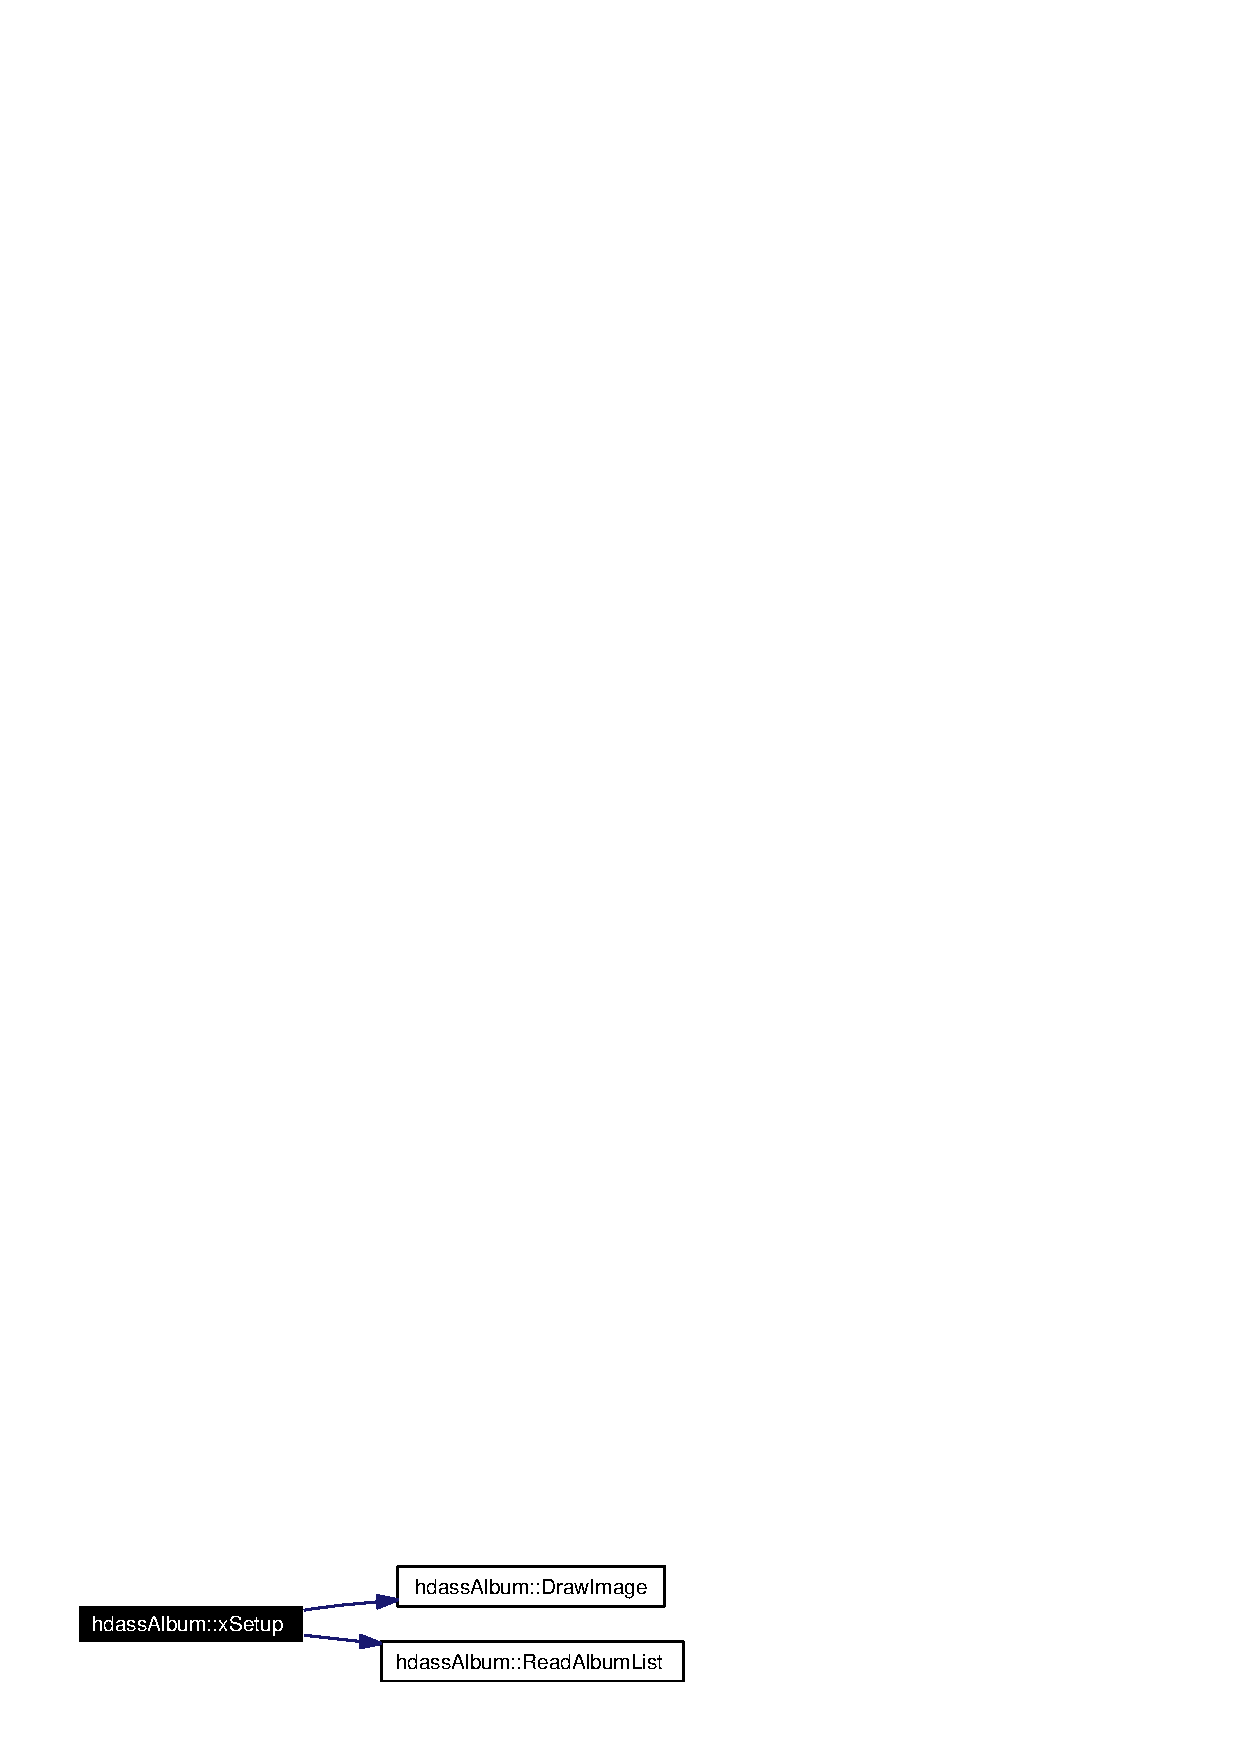
\includegraphics[width=164pt]{classhdassAlbum_ImageDetiala2_cgraph}
\end{center}
\end{figure}


\subsection{Member Data Documentation}
\index{ImageDetial@{Image\-Detial}!AlbumList@{AlbumList}}
\index{AlbumList@{AlbumList}!ImageDetial@{Image\-Detial}}
\subsubsection{\setlength{\rightskip}{0pt plus 5cm}KURL::List {\bf hdass\-Album::Album\-List}\hspace{0.3cm}{\tt  [inherited]}}\label{classhdassAlbum_ImageDetialo1}




Definition at line 50 of file hdassalbum.h.

Referenced by hdass\-Album::Add\-Image\-To\-Album(), hdass\-Album::Read\-Album\-List(), hdass\-Album::Remove\-Image\-From\-Album(), hdass\-Album::slot\-Next\-Image(), and hdass\-Album::slot\-Previous\-Image().\index{ImageDetial@{Image\-Detial}!FloderList@{FloderList}}
\index{FloderList@{FloderList}!ImageDetial@{Image\-Detial}}
\subsubsection{\setlength{\rightskip}{0pt plus 5cm}KURL::List {\bf hdass\-Album::Floder\-List}\hspace{0.3cm}{\tt  [inherited]}}\label{classhdassAlbum_ImageDetialo2}




Definition at line 50 of file hdassalbum.h.\index{ImageDetial@{Image\-Detial}!it@{it}}
\index{it@{it}!ImageDetial@{Image\-Detial}}
\subsubsection{\setlength{\rightskip}{0pt plus 5cm}KURL::List::Const\-Iterator {\bf hdass\-Album::it}\hspace{0.3cm}{\tt  [inherited]}}\label{classhdassAlbum_ImageDetialo0}




Definition at line 49 of file hdassalbum.h.

Referenced by hdass\-Album::Read\-Album\-List(), hdass\-Album::slot\-Next\-Image(), and hdass\-Album::slot\-Previous\-Image().\index{ImageDetial@{Image\-Detial}!PixList@{PixList}}
\index{PixList@{PixList}!ImageDetial@{Image\-Detial}}
\subsubsection{\setlength{\rightskip}{0pt plus 5cm}QPtr\-List$<$QPixmap$>$ {\bf hdass\-Album::Pix\-List}\hspace{0.3cm}{\tt  [inherited]}}\label{classhdassAlbum_ImageDetialo3}




Definition at line 51 of file hdassalbum.h.

The documentation for this class was generated from the following files:\begin{CompactItemize}
\item 
{\bf imagedetial.h}\item 
{\bf imagedetial.cpp}\end{CompactItemize}
